% Specifies the document class. '11pt' sets the font size.
\documentclass[10pt]{article}

% --- PACKAGE IMPORTS ---
\usepackage{amsmath}        % For advanced math typesetting
\usepackage{amssymb}        % For additional math symbols
\usepackage{graphicx}       % To include images
\usepackage[margin=1in]{geometry} % To set page margins
\usepackage{hyperref}       % For clickable links (URLs, references)
\usepackage{authblk}        % For author affiliations
\usepackage{enumitem}       % For customized lists
\usepackage{algorithm}      % For algorithm environment
\usepackage{algpseudocode}  % For pseudocode
\usepackage{booktabs}       % For nicer tables
\usepackage{tabularx}
\setlength{\columnsep}{20pt} % Default is 10pt. Try 15pt, 20pt, or 25pt.

\twocolumn

% --- DOCUMENT METADATA ---
\title{%
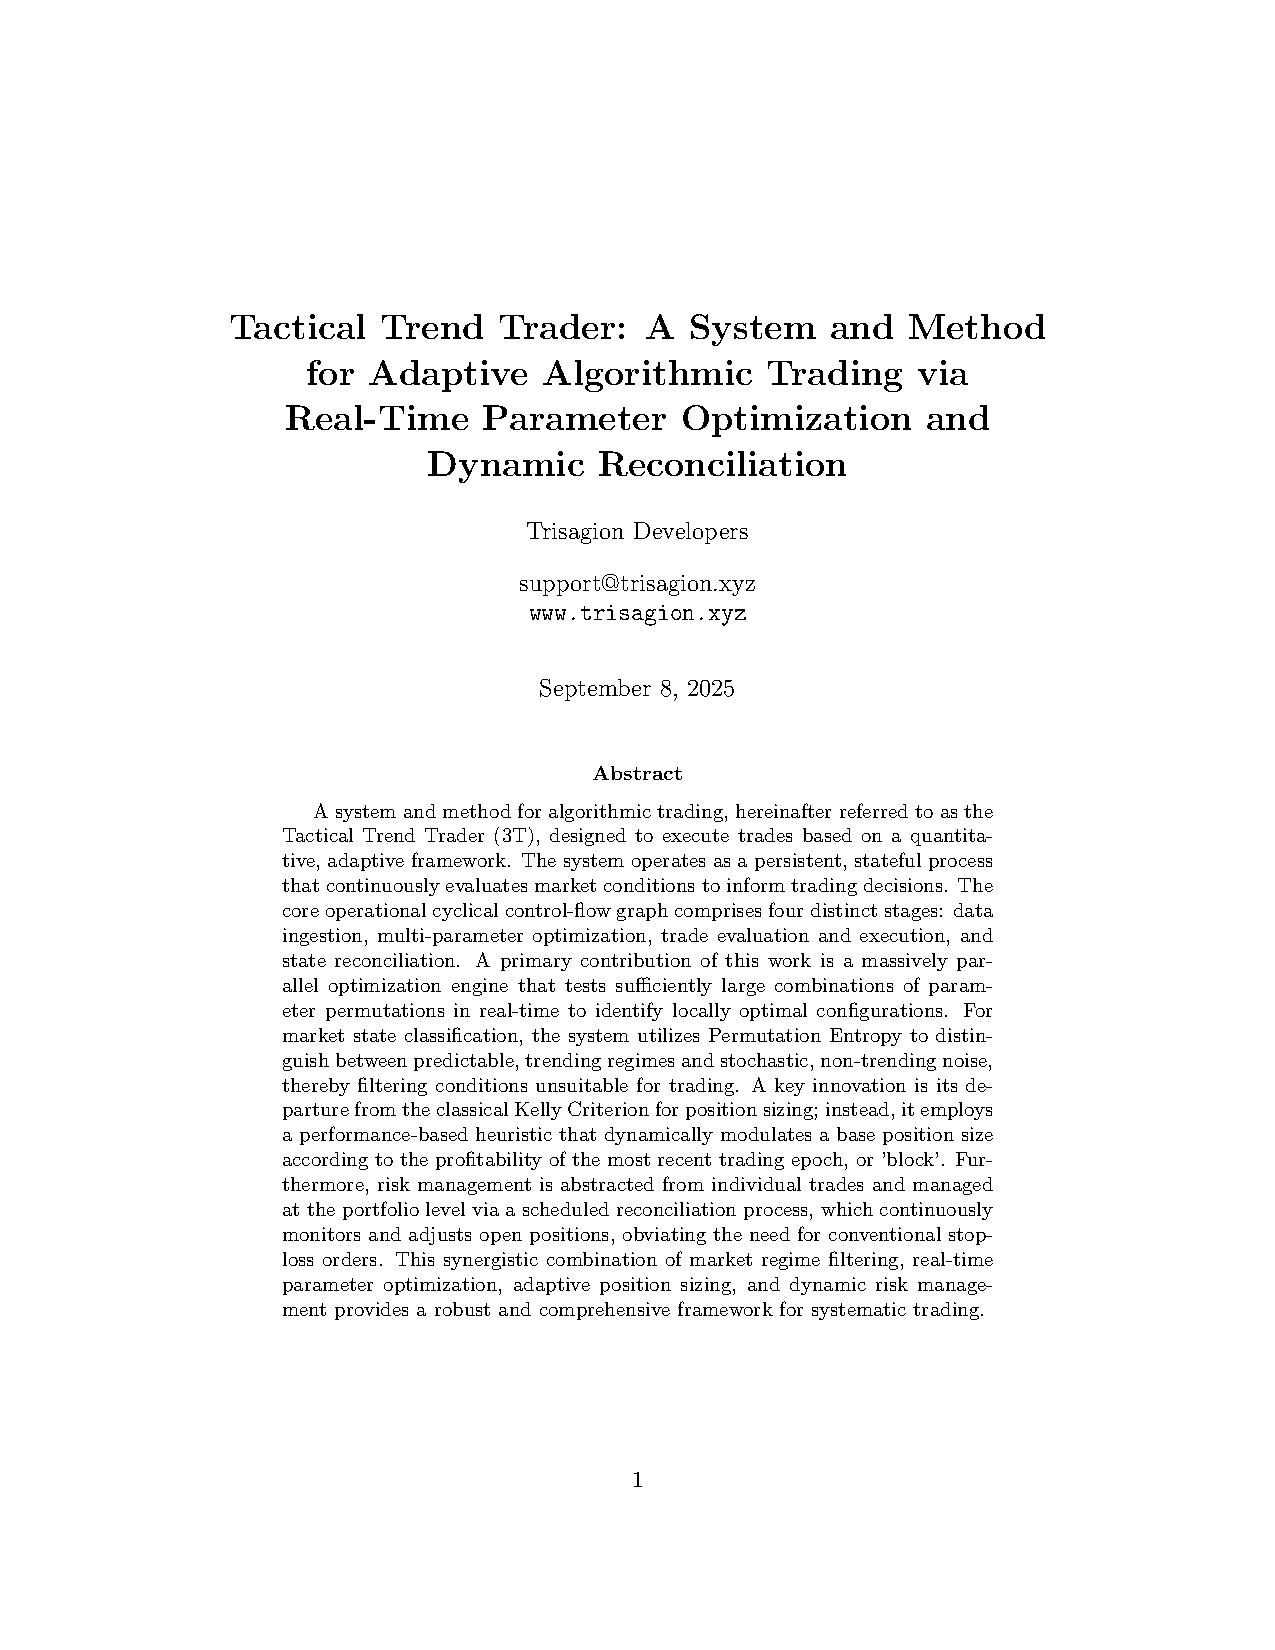
\includegraphics[width=2.5cm]{TTT.pdf}

\textbf{Tactical Trend Trader: A System and Method for Adaptive Algorithmic Trading via Real-Time Parameter Optimization and Dynamic Reconciliation}}
\author{Trisagion Developers \\
        \href{mailto:support@trisagion.xyz}{support@trisagion.xyz} \\
        \url{www.trisagion.xyz}}
\date{\today}

% --- BEGIN DOCUMENT ---
\begin{document}

\maketitle


% --- ABSTRACT ---
\begin{abstract}
    A system and method for algorithmic trading, hereinafter referred to as the Tactical Trend Trader (3T), designed to execute trades based on a quantitative, adaptive framework. The system operates as a persistent, stateful process that continuously evaluates market conditions to inform trading decisions. The core operational cyclical control-flow graph comprises four distinct stages: data ingestion, multi-parameter optimization, trade evaluation and execution, and state reconciliation. A primary contribution of this work is a massively parallel optimization engine that tests sufficiently large combinations of parameter permutations in real-time to identify locally optimal configurations. For market state classification, the system utilizes Permutation Entropy to distinguish between predictable, trending regimes and stochastic, non-trending noise, thereby filtering conditions unsuitable for trading. A key innovation is its departure from the classical Kelly Criterion for position sizing; instead, it employs a performance-based heuristic that dynamically modulates a base position size according to the profitability of the most recent trading epoch, or 'block'. Furthermore, risk management is abstracted from individual trades and managed at the portfolio level via a scheduled reconciliation process, which continuously monitors and adjusts open positions, obviating the need for conventional stop-loss orders. This synergistic combination of market regime filtering, real-time parameter optimization, adaptive position sizing, and dynamic risk management provides a robust and comprehensive framework for systematic trading.
\end{abstract}

% --- INTRODUCTION ---
\section{Introduction}
The domain of algorithmic trading is characterized by a persistent challenge: developing systems that can adapt to non-stationary and often chaotic financial markets. Many conventional systems rely on statically configured parameters, rendering them brittle and susceptible to performance degradation as market dynamics shift. The Tactical Trend Trader (3T) is a computer-implemented system engineered to address these limitations by integrating real-time adaptability into its core architecture. It is designed to optimize performance by leveraging statistical analysis for market regime detection and a novel set of heuristics for risk and position management.

Early system development focused on a regression based dual-state cycle with training data produced through a fresh set of continuously generated instances of feature values, that was utilized in bootstrap aggregated ensembles and then validated with k-fold cross validation. During inference a run would only execute against live risk if the predictor scored positively in terms of expected profit and loss of the run. Over the period of several months of study, the inference set consistently underperformed the same training data if it was left to execute against risk so randomized out of sample feature values were superior to carefully trained tabular predictors. Although an early advantage was observed via inference for short term profitability it was always underperforming over longer timeframes. Since most of the value is captured when the system can catch a trend, any short term advantage observed decreased over time so the machine learning aspect was removed entirely. 

The 3T system operates in a continuous loop, analyzing market data to first identify predictable, trending environments and then deploying capital with a position size dynamically calibrated to recent system performance. This paper details the mathematical framework, system architecture, and unique operational logic of the 3T. The primary contributions of this method are threefold:
\begin{enumerate}
    \item \textbf{A Real-Time Optimization Engine:} A mechanism that continuously stress-tests sufficiently large numbers of parameter permutations against live market data to inform the primary trading algorithm.
    \item \textbf{A Hybrid Risk Management Model:} A novel heuristic for position sizing based on recent performance, coupled with a dynamic, reconciliation-based approach to position control that replaces static, per-trade stop-losses.
    \item \textbf{Dual Entry Logic:} A configurable system that supports both momentum-following ("breakout")\cite{lefevre1923} and mean-reverting ("swing")\cite{taylor1950} entry strategies simultaniously, allowing for greater tactical flexibility.
\end{enumerate}

% --- SYSTEM ARCHITECTURE ---
\section{System Architecture}
The 3T system is a modular architecture comprising four main components: a Data Ingestion Module, a Parameter Optimization Engine, a Trade Evaluation and Execution Engine, and a State Reconciliation Module. This separation of concerns ensures robustness and scalability.

\subsection{Data Ingestion Module}
This module serves as the sensory input for the entire system, acquiring market data from two primary sources:
\begin{itemize}
    \item \textbf{Real-time Websocket Stream:} Provides low-latency access to immediate price updates (tick data), crucial for the Parameter Optimization Engine.
    \item \textbf{Historical API Endpoint:}: Fetches historical Open/High/Low/Close (OHLC) data, which is subsequently aggregated into one-minute volatility bars. This provides the necessary historical context for macro-level analysis like Permutation Entropy calculation based on large amounts of summarized data instead of looking at individual ticks.
\end{itemize}
The module includes logic for data normalization, cleaning, and ensuring data integrity before it is passed to the analytical engines.

\subsection{Parameter Optimization Engine}
This engine operates as a continuous, massively parallel simulation layer that runs concurrently with the live trading system. Its purpose is to find the most profitable set of parameters for the core trading algorithm in the current market environment strickly as a function of out of sample performance. It cyclically tests sufficiently large numbers of permutations of a core set of variables against real-time data to determine the most profitable configurations. The key parameters under optimization include:
\begin{itemize}
    \item \textbf{Permutation entropy parameters:} The embedding dimension $d$ and time lag $\tau$ used for market state analysis.
    \item \textbf{Market state thresholds:} The specific value of Permutation Entropy, $H_{trend}$, below which the market is considered 'trending'.
    \item \textbf{Max duration:} The maximum time, in seconds, that a single simulation (a 'run') is allowed to process data before it is terminated. This constrains the computational search space.
    \item \textbf{Max direction reversal:} The maximum time, in seconds, that a run will attempt to find a market direction before exiting. This parameter helps manage risk exposure during periods of indecisive price action.
    \item \textbf{APR target:} The target Annual Percentage Rate (APR) that the system aims to achieve. This serves as a benchmark for performance evaluation and the fitness function of the optimization.
    \item \textbf{Rolling APR minutes:}: The time window, in minutes, over which the system's APR is calculated. This determines the sensitivity of the system to recent performance.
    \item \textbf{Decision distance seconds:}: The minimum time interval between successive trade evaluations to allow for the maturation of the market's response to the previous action to avoid noise in the APR curve.
    \item \textbf{System type:}: The fundamental entry logic, supporting "breakout" or "swing" methodologies.
\end{itemize}
The most profitable feature values for a given run instance discovered by this engine is then propagated to the Trade Evaluation and Execution Engine to be used in the live risk-on environment.

% --- MATHEMATICAL FRAMEWORK AND OPERATIONAL LOGIC ---
\section{Mathematical Framework and Operational Logic}
The core of the 3T is a continuous loop executed by the Trade Evaluation and Execution Engine, which acts upon the optimal parameters supplied by the Parameter Optimization Engine. Each iteration performs a rigorous sequence of data analysis and trade management operations.

\subsection{Market Regime Analysis via Permutation Entropy}
To prevent trading in stochastic, unpredictable market conditions, the system first performs a market regime analysis. This methodology is chosen for its robustness to noise and its model-free nature.\cite{PhysRevLett.88.174102}
\begin{enumerate}
    \item A time series is constructed from the most recent $N$ price points derived from the aggregated volatility bars.
    \item Permutation Entropy, $H(d)$, is calculated on this time series using the optimized parameters ($d$, $\tau$). The formula for Permutation Entropy is given by:
    $$ H(d) = -\sum_{i=1}^{d!} p_i \log_2 p_i $$
    where $d$ is the embedding dimension and $p_i$ is the relative frequency of the $i$-th permutation ordinal pattern.
    \item If the calculated value $H(d)$ is below the optimized threshold $H_{trend}$, the market is classified as \textbf{trending} and algorithmically has a higher skew towards predictable behavior. The algorithm proceeds to the next stage. Otherwise, the market is classified as \textbf{noisy}, and no new trading action is initiated.
\end{enumerate}

\subsection{System Entry Logic: Breakout and Swing Types}
Once a trending market is confirmed, the system employs its configured entry logic based on the system\_type parameter.
\begin{itemize}
    \item \textbf{Breakout Logic:} This is a momentum-following strategy. For example, a long entry is considered if the current price exceeds the highest high of the last $N$ periods, and a short entry is considered if the price falls below the lowest low of the last $N$ periods. This logic seeks to capitalize on the continuation of a strong trend.
    \item \textbf{Swing Logic:} This is a mean-reversion strategy. It identifies short-term price extensions away from a central tendency (e.g., a moving average). A long entry is considered when the price has dipped significantly below the mean and shows signs of reverting, while a short entry is considered after a significant rally above the mean. This provies a "trigger premium" benefit to the entry by capturing the trend at a more favorable entry point.
\end{itemize}

\subsection{Position Sizing Heuristic and APR Trend Analysis}
When a valid entry signal is generated, the system determines whether to increase its risk exposure. This decision is governed by a strict gating condition based on the system's profitability trend, as measured by its Annual Percentage Rate (APR), calculated over the rolling APR minutes window.

\subsubsection{APR Gating Condition}
A core rule of the risk management framework is that position size will \textbf{only} be increased if the system's rolling APR is trending positively and is above the APR target. If the APR is flat, negative, or below target, the system will not increase its base position size, ensuring that risk is escalated only during periods of sustained, proven time normalized profitability.

\subsubsection{Performance‑Based Sizing Heuristic}
If the APR gating condition is met, the system calculates the appropriate position size. It deliberately eschews a direct implementation of the Kelly Criterion\cite{kelly1956new,tharpinstitute_peak}, which can be sensitive to estimation errors in probabilities and payoffs. Instead, it employs a novel performance‑based heuristic that modulates a base risk position size ($S_{\text{base}}$) based on the performance of the current run instance ('top or null block height', $H_{\text{top}}$).

The performance factor, $P_{\text{kelly}}$, is now defined as a **relative change** between the Kelly percentages of the current (height = NULL) runs and the historical (height ≠ NULL) runs:

\begin{equation}
\label{eq:kelly-performance}
P_{\text{kelly}} =
\begin{cases}
0, & H_{\text{hist}} = 0 \\[6pt]
\displaystyle
\frac{H_{\text{cur}} - H_{\text{hist}}}{\lvert H_{\text{hist}} \rvert},
& \text{otherwise}
\end{cases}
\end{equation}

where:
\begin{itemize}
    \item $H_{\text{cur}}$ is the Kelly percentage computed from runs with \texttt{height IS NULL}.
    \item $H_{\text{hist}}$ is the Kelly percentage computed from runs with \texttt{height IS NOT NULL}.
\end{itemize}

The factor $P_{\text{kelly}}$ is then **clipped** to a symmetric bound $[-\tau,\tau]$ (default $\tau = 0.5$) and additionally **floored** at $-0.98$ to avoid a sign reversal that would otherwise flip the position direction. The final position size is obtained by applying the bounded performance factor to the base risk size:

\begin{equation}
\label{eq:kelly-adjusted}
S_{\text{final}} = S_{\text{base}} \bigl(1 + \operatorname{clip}(P_{\text{kelly}}, -\tau, \tau)\bigr)
\end{equation}

\paragraph{Derivation \& Edge‑Case Handling}
The following table summarises how edge cases observed in production are handled both in code and in the mathematical description:

% This is the corrected version
\begin{table*}[t] % Use [t] for top or [b] for bottom placement, [h] is often ignored for table*
\small
\centering
\caption{Edge‑case handling for the Kelly‑based performance factor.}
\label{tab:edge-cases} % It's good practice to add a label for referencing
\begin{tabularx}{\textwidth}{@{} l l >{\raggedright\arraybackslash}X @{}} % <-- THE FIX IS HERE
\toprule
\textbf{Edge case} & \textbf{Handling in code} & \textbf{Paper description} \\ \midrule
$H_{\text{hist}} = 0$ (no historical data) & Return base size unchanged & “If no historical Kelly can be computed, the engine falls back to the unadjusted base size.” \\
Insufficient sample size $<10$ runs & Return \texttt{None} → fallback & “Kelly is only calculated when at least ten qualifying runs exist; otherwise the metric is unavailable.” \\
$|P_{\text{kelly}}| > \tau$ & Clip to $\pm\tau$ & “A hard cap prevents runaway position scaling.” \\
$P_{\text{kelly}} < -1.0$ & Floor at $-0.98$ & “The floor avoids a sign reversal that would otherwise flip the position direction.” \\
\bottomrule
\end{tabularx}
\end{table*}

\paragraph{Algorithmic Pseudocode}
Algorithm~\ref{alg:kelly-sizing} presents the high‑level steps executed by the reconciliation engine.

\begin{algorithm}[H]
\caption{Kelly‑adjusted position sizing}
\label{alg:kelly-sizing}
\begin{algorithmic}[1]
\State $H_{\text{cur}} \gets$ \texttt{\_calculate\_kelly\_metrics(..., ``height IS NULL'')}
\State $H_{\text{hist}} \gets$ \texttt{\_calculate\_kelly\_metrics(..., ``height IS NOT NULL'')}
\If{$H_{\text{cur}}$ is \texttt{None} \textbf{or} $H_{\text{hist}}$ is \texttt{None}}
    \State $S_{\text{final}} \gets S_{\text{base}}$
\Else
    \State $P \gets \dfrac{H_{\text{cur}} - H_{\text{hist}}}{\lvert H_{\text{hist}} \rvert}$
    \State $P \gets \operatorname{clip}(P,\ -\tau,\ \tau)$
    \State $S_{\text{final}} \gets S_{\text{base}} \times (1 + P)$
\EndIf
\State \Return $S_{\text{final}}$
\end{algorithmic}
\end{algorithm}

\subsubsection{Bootstrapping Logic}
Upon initial deployment, the system exists in a "cold start" state with no historical block heights to inform the sizing heuristic. To mitigate this, the system uses a pre‑configured, conservative default position size for its first trade. Once this initial target is achieved, its resulting profit or loss establishes the first block height ($height = 1$). This value, along with subsequent block heights, forms the statistical basis for the benchmark $B_{\text{kelly}}$, enabling the heuristic for all future trades.

\subsubsection{Execution and Risk Management}
\begin{enumerate}
    \item \textbf{Take‑Profit}: A take‑profit goal is considered at a pre‑configured, fixed percentage gain from the portfolio value at start of the current block. When the orders are executed, the positions are closed, and the realized active runs are recorded as part of the newest block height.
    \item \textbf{Risk Management}: A key innovation of the 3T is its explicit omission of traditional, per‑trade stop‑loss orders, which are often susceptible to being triggered by transient market volatility or "stop hunting." Instead, risk is managed holistically through continous State Reconciliation.
\end{enumerate}

% --- STATE RECONCILIATION MODULE ---
\section{State Reconciliation Module}
The State Reconciliation Module functions as a dynamic, portfolio‑level risk manager. Its operation is not event‑driven by price action but is scheduled to run at a configured interval (e.g., every 10 minutes). This prevents high‑frequency, reactive adjustments and allows positions time to mature.

During each reconciliation cycle, the module assesses the aggregate health of all open positions. It references the ongoing simulations within the Parameter Optimization Engine to determine the expected performance of the current live configuration. If the actual portfolio performance deviates significantly from the simulated expectancy, or if the market regime has shifted to 'noisy', the module takes corrective action based on the simulated success value of the permutation. This may involve partially reducing a position to decrease exposure or closing a position entirely, even if its take‑profit level has not been reached.

To prevent excessive trading fees from minor adjustments ("churn"), the module will only execute a change if the required adjustment in position size is above a minimum financial or percentage threshold (e.g., \$100 or 1.5\% of the account's total equity). This ensures that only strategically meaningful risk adjustments are made, serving as an intelligent, system‑wide stop‑loss mechanism. 

In order to apply risk changes only when the relability of the current risk‑on positions are sound, multiple oberver nodes are utilized to ensure consensus.\cite{lamport1982byzantine} This prevents the situation of a runaway process continously adding or removing from a position without checks, balances and reconciliations at each iteration.

% --- CONFIGURATION PARAMETERS ---
\section{Configuration Parameters}
The reconciliation engine is driven by a small set of runtime configuration keys. Table~\ref{tab:config} lists the keys, their defaults, and a brief description.

\begin{table*}[t] % Changed [h] to [t] for better placement
\small
\centering
\caption{Key configuration parameters used by the reconciliation engine during testing.}
\label{tab:config}
% The only change is in the line below
\begin{tabularx}{\textwidth}{@{} l l >{\raggedright\arraybackslash}X @{}}
\toprule
\textbf{Config key} & \textbf{Default} & \textbf{Meaning} \\ \midrule
\texttt{kelly\_threshold} & $0.5$ & Symmetric cap for the performance factor $P_{\text{kelly}}$. \\
\texttt{risk\_pos\_percentage} & $0.0016180339887$ & Fraction of account equity used as the base risk size. \\
\texttt{minimum\_trade\_threshold} & $20.0$ (USD) & Minimum notional size before a trade is emitted. \\
\texttt{position\_staleness\_timeout} & $300$\,s & Max age of a local position record before it is considered stale. \\
\end{tabularx}
\end{table*}

% --- CONCLUSION ---
\section{Conclusion}
The Tactical Trend Trader (3T) provides a robust and complete framework for adaptive algorithmic trading. Its novelty lies in the synergistic combination of its core components: (1) the use of Permutation Entropy for robust market regime filtering, (2) a massively parallel, real‑time Parameter Optimization Engine that ensures the system remains adapted to current market dynamics, (3) a unique performance‑based heuristic for dynamic position sizing, and (4) an active reconciliation module for portfolio‑level risk management that replaces brittle, traditional stop‑loss orders.

By systematically filtering for predictable market environments, continuously optimizing its own parameters, and intelligently adjusting risk based on real‑time performance and expected outcomes, the 3T system is designed to navigate complex financial markets, with the objective of maximizing risk‑adjusted returns while diligently managing downside exposure.

% --- FUTURE WORK / OPEN ISSUES ---
\section{Future Work \& Open Issues}
The earlier implementation suffered from sign‑flipping when the current and historical Kelly values straddled zero. By switching to the relative‑change metric (Eq.~\ref{eq:kelly-performance}) the sign is now intrinsic, eliminating the need for ad‑hoc \texttt{*‑1} corrections. Future work includes exploring a Bayesian‑shrinkage estimator for Kelly to further stabilise the metric when sample sizes are low, and extending the configuration schema to allow per‑symbol thresholds.

% --- REFERENCES ---
\begin{thebibliography}{9}

\bibitem{PhysRevLett.88.174102}
Christoph Bandt and Bernd Pompe,
\textit{Permutation Entropy: A Natural Complexity Measure for Time Series},
Phys. Rev. Lett. \textbf{88}, 174102 (2002).

\bibitem{kelly1956new}
J. L. Kelly, Jr.,
\textit{A New Interpretation of Information Rate},
Bell System Technical Journal, \textbf{35}(4), 917-926 (1956).

\bibitem{lamport1982byzantine}
Leslie Lamport, Robert Shostak, and Marshall Pease,
\textit{The Byzantine Generals Problem},
ACM Transactions on Programming Languages and Systems, \textbf{4}(3), 382-401 (1982).

\bibitem{tharpinstitute_peak}
Van Tharp Institute,
\textit{Peak Performance 101 Course for Traders and Investors}.
Available online: \url{https://vantharpinstitute.com/course/peak-performance-course-for-traders-and-investors/}.
(Accessed on: September 8, 2025).

\bibitem{taylor1950}
George Douglas Taylor,
\textit{The Taylor Trading Technique},
self-published (1950).

\bibitem{lefevre1923}
Edwin Lefèvre,
\textit{Reminiscences of a Stock Operator},
George H. Doran Company (1923).

\end{thebibliography}

\end{document}
